\chapter{Experiment 1: Optimal spatial resolution for BOLD fMRI decoding analyses at \sevenT}


%\linenumbers
\section*{Introduction}

The term multivariate pattern (MVP) analysis summarizes a range of data
analysis strategies that are highly suitable for studying neural
representations encoded in distributed patterns of brain activity
\citep{haxby_2012}. While there is an ever increasing number of publications
that demonstrate the power of MVP analysis for functional magnetic resonance
imaging (fMRI) data \citep{opdebeeck_2010,freeman_2011,alink_2013,freeman_2013}
with standard resolution data (a voxel size of about \mm{2-3} isotropic), MVP
analysis is especially promising in the context of high-resolution fMRI.
Ongoing technological improvements, such as ultra high-field MRI scanners
(\sevenT\ or higher) have pushed the resolution for fMRI to a level
that is slowly approaching the spatial scale of the columnar organization of
the brain \citep{yacoub_2008,heidemann_2012}. Being able to use fMRI to sample
brain activity patterns at a near-columnar level makes it feasible to employ
MVP analysis with the aim to decode distributed neural representations of an
entire cortical field at a level of detail that is presently only accessible to
invasive recording techniques with limited spatial coverage. However, at this
point, it is unclear which spatial resolution is most suitable for decoding
neural representation from fMRI data with MVP analysis. While higher
resolutions can improve the fidelity of the BOLD signal by, for example,
reducing the partial volume effect \citep{Weibull_2008}, the benefits can be
counteracted by physiological noise (such as inevitable motion) and lower tSNR. 
This raises the question: does the decoding of neural representations continuously improve
with increasing spatial resolution, or is there an optimal resolution for a
given type of representation?

In this study, we aim to address this question for the most frequently employed
MVP analysis technique: a cross-validated classification analysis, where a
classifier is repeatedly trained to distinguish patterns of brain activation
from fMRI data of a set of stimulus conditions, and its prediction accuracy is
evaluated against a left-out data portion \citep{pereira_2009}. Moreover, we
focus on the decoding of the representation of oriented visual gratings in
primary visual cortex. This is likely to be the most extensively studied
paradigm regarding the application of MVP analysis on fMRI data, starting with
the classic studies of  \citet{kamitani_2005} and \citet{haynes_2005}. It was
shown that orientation can be decoded reliably at resolutions ranging from
standard \mm{3} isotropic voxels in the aforementioned studies, to \mm{1}
\citep{swisher_2010}, and that it is possible to directly measure orientation
columns in V1 with \sevenT\ fMRI of \mm{0.5$\times$0.5} (in-plane) resolution
\citep{yacoub_2008,ugurbil_2012}. These findings led to a debate on the origin
and the spatial scale of the signals that classifiers can use to learn to
discriminate different orientations
\citep{opdebeeck_2010,swisher_2010,alink_2013,freeman_2013}. To investigate
these questions, the authors typically acquired high-resolution fMRI and
simulated a lower-resolution acquisition by applying spatial filters to the
original data in order to compare metrics, such as prediction accuracy, across
a range of spatial frequencies \citep[see][]{swisher_2010}.  However, this
approach has not gone unchallenged as it is unclear to what degree particular
filtering strategies \citep[e.g. Gaussian filtering vs. low-pass filtering in
the spatial frequency domain, see][]{misaki_2013} can effectively simulate the
properties of fMRI recorded at a lower physical resolution, where a change in
slice thickness alone can significantly alter image contrast. Despite this
criticism, we are not aware of any study that has compared the performance of
orientation decoding in visual cortex across a range of physical acquisition
resolutions.

In this study, we provide empirical data on the effect of spatial acquisition
resolution on the decoding of visual orientation from high field (\sevenT)
fMRI. We recorded BOLD fMRI data at \mm{0.8}, \mm{1.4}, \mm{2} and \mm{3} voxel
size while participants were visually stimulated with oriented phase-flickering
gratings using a uniform event-related paradigm.
% optimal resolution
These data enable estimation of the \textit{optimal acquisition resolution} for
orientation decoding from \sevenT\ fMRI.  \citet{chaimow_2011} investigated the
decoding of the stimulated eye using simulated \threeT\ fMRI data based
on a model of ocular dominance columns. They found that a resolution of \mm{3}
was optimal for decoding and performance decreased with higher or lower
resolution.  As it is known that in monkeys the organization of orientation
columns is characterized by higher spatial frequencies than ocular dominance
columns \citep{obermayer_1993}, we expect any optimal resolution for
orientation decoding to be higher than \mm{3}. Moreover, the BOLD point-spread
function (PSF) at \sevenT\ is known to be considerably smaller than at \threeT\
\citep[\mm{$\approx$2.3} FWHM vs.  \mm{$\approx$3.5} FWHM][]{shmuel_2007,
engel_1997} which should further increase the optimal resolution for decoding
at \sevenT.
% filtering
Multi-resolution data also allow for evaluating \textit{filtering strategies}
used in previous studies in terms of their validity regarding the simulation of
lower-resolution fMRI acquisitions from high-resolution data.
% aliasing
These data also enable the investigation of the \textit{role of aliasing} of a
high spatial-frequency signal (beyond the Nyquist frequency) into a
lower frequency range sampled by fMRI voxels \citep[sometimes referred to as
“hyperacuity”;][]{swisher_2010,opdebeeck_2010}, as, in the case of spatial
aliasing, the frequency bands carrying an orientation-selective signal would
vary with the sampling resolution of fMRI.
% veins
Lastly, we collected high-resolution susceptibility weighted imaging data for
blood-vessel localization in order to investigate the \textit{role of large
draining veins} that may carry orientation-selective signals reflected in low
spatial frequency components when sampled by millimeter range voxels
\citep{kamitani_2005,kriegeskorte_2007,shmuel_2010, gardner_2010}. In
combination with the multi-resolution fMRI data, we can investigate the effect
of this potential signal source on the orientation decoding at various levels
of spatial scale.



\section*{Materials and methods}

\subsection*{Participants}

\noindent Seven healthy right-handed volunteers (age \unit[21-38]{years}, 5
males) with normal or corrected to normal vision were paid for their
participation. Before every scanning session, they were provided with
instructions for the experiment and signed an informed consent form. The study
was approved by the Ethics Committee of the Otto-von-Guericke University.

\subsection*{Stimuli}

\noindent A stimulus comprised two semi-annular patches of flickering sine-wave
gratings left and right of a central fixation point on a medium gray background
(0.8\textdegree-7.6\textdegree\ eccentricity, 160\textdegree\ width on each
side with a 20\textdegree\ gap along the vertical meridian, above and below the
fixation point, to aid separation of gratings between hemifields). Gratings on
each side of the stimulus were independently oriented at either 0\textdegree,
45\textdegree, 90\textdegree, or 135\textdegree, with a constant spatial
frequency of 1.4 cycles per degree of visual angle corresponding to the 
center of the screen, a contrast of 100\%, and a flickering frequency of 
\unit[4]{Hz} with 50\% duty cycle \citep[][]{swisher_2010}. The phase of the
gratings was changed at a frequency of \unit[4]{Hz} and was chosen randomly
from 0, $\frac{\pi}{2}$, $\pi$, or $\frac{3\pi}{2}$ degrees of phase angle
(Figure~\ref{fig:exp_design}).

Stimulus presentation and response logging were implemented using PsychoPy
\citep[v1.79; ][]{peirce_2008} running on a computer with the (Neuro)Debian
operating system \citep{HH12}. Stimuli were displayed on a rear-projection
screen (1280$\times$1024 pixels resolution; \unit[60]{Hz} video refresh rate;
\unit[25.5]{cm} wide) located behind the head coil. Participants viewed the
screen via a mirror placed at a distance of \unit[$\approx$4]{cm} from their
eyes. The total viewing distance was \unit[100]{cm}.

\subsection*{Behavioral task}

\noindent In order to keep the participants' attention focused and to minimize
eye-movements, they performed a reading task that was unrelated to the
stimulation with oriented gratings. A black circle (radius 0.25\textdegree) was
presented as a fixation point at the center of the screen. Within this circle,
a randomly selected excerpt of song lyrics was shown as a stream of single letters
(0.3\textdegree\ height, letter frequency \unit[2]{Hz}) throughout the entire
length of a run. Each trial started with \seconds{3} of stimulation with
oriented gratings and continued for another \seconds{5} of a task-only period
(Figure~\ref{fig:exp_design}). During task-only periods, a medium gray
background was displayed in both hemifields. At the end of each run, the
participant was asked a question related to the previously read text.

In a pilot experiment with in-scanner eye-movement recordings, the letter
reading task was found to minimize eye-movements effectively; however, it was
unsuitable to verify fixation accuracy on a trial-by-trial basis. In order to
evaluate a potential impact of the reading task on the orientation decoding
performance, the task was replaced for one participant with a visual detection
task. One participant was repeatedly presented with a Landolt C stimulus
(radius 0.12\textdegree, left or right opening (0.048\textdegree) at random
intervals in each run. The participants had to respond to the direction of the
opening of the probe by pressing one of two buttons corresponding to a left or
right opening. Discrimination accuracy for this participant was 98.6\%, while
orientation decoding performance did not qualitatively differ from mean
decoding accuracy of other participants. The performance of the subject with the Landolt C 
task was compared relative to the 95\% binomial proportion 
confidence interval computed from the number of correct predictions (BOLD pattern classification), 
concatenated across hemispheres and cross-validation fold, and all subjects performing the 
reading task. For all resolutions but 3\mm the performance of the subject 
performing the Landolt C task was close to the lower boundary of the 
confidence interval, for 3\mm it was close to the upper boundary. This suggests that the
employed reading task was effective in keeping participants focused on the
fixation point.

\begin{figure}
  \centering
  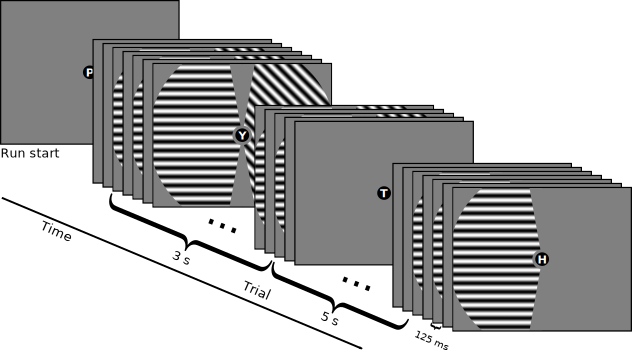
\includegraphics[width=\linewidth]{figure_1}

  \caption{
    %
    Stimulation paradigm. Independent flickering oriented grating stimuli on a
    medium gray background were presented in both hemifields for \seconds{3} at
    the beginning of each trial. Stimulation was followed by a \seconds{5}
    inter-trial interval. Throughout an entire experiment run, participants
    performed a continuous central letter reading task to maintain fixation.
    Interspersed trials where the previous stimulus was repeated in only one of
    the hemifields were used to decouple stimulation sequences.
  %
  }

  \label{fig:exp_design}
\end{figure}

\subsection*{Procedures}

\noindent Participants were scanned in five different sessions, one experiment
session for each of the four acquisition resolutions (\mm{0.8}, \mm{1.4},
\mm{2.0} and \mm{3.0} isotropic) and one session for retinotopic mapping. These
sessions took place on different days over the course of five weeks. The order
of acquisition resolutions was randomized for each participant. In every
experiment session, participants completed ten runs with short breaks
in-between, without leaving the scanner. Each run comprised \unit[30]{trials}
(\seconds{8} duration; \unit[4]{min} total run duration). In 20 of these
trials, a combination of oriented gratings, one in each hemifield, was presented
simultaneously so that each of the four orientations occurred exactly five
times in each hemifield. The sequence of orientations was independently
randomized for each hemifield, resulting in random pairings of orientations
within trials. In order to decouple stimulation sequences between hemifields,
ten NULL events were inserted into the trial sequence at pseudo-random
positions (a run could not start with a NULL event and no two NULL events
could occur in immediate succession). NULL events were identical to regular
trials, except for the fact that in one hemifield the same oriented grating as
in the previous trial was repeated while the other hemifield remained empty.
The side of the blank hemifield was chosen at random for each NULL event. For
all participants, the actual generated trial sequences show a roughly equal
count of NULL events for each hemifield and frequency of unique combinations of
grating orientations (refer to supplementary Figure~\ref{fig:ipsi} for more details). 

\subsection*{Functional imaging}
\noindent The objective for functional data acquisition was to obtain BOLD fMRI
data from the V1 ROI at four different resolutions with an identical
stimulation paradigm. MR acquisition parameters were chosen to be maximally
similar across resolutions given two a priori constraints: 1) sufficient
spatial coverage of the V1 ROI and 2) identical sampling frequency (TR) across
resolutions.

T2*-weighted echo planar images (EPI) (TR/TE=\unit[2000/22]{ms},
FA=90\textdegree) of the occipital lobe were acquired during visual stimulation
using a \sevenT\ whole body scanner (Siemens, Erlangen, Germany) and a 32
receive channel head coil (Nova Medical, Wilmington, MA). Slices, oriented
parallel to the calcarine sulcus (on a tilted axial plane), were acquired for 4
different spatial resolutions, i.e. \mm{3} isotropic (FoV=\mm{198}, matrix
size 66$\times$66, 37 slices, GRAPPA accel.~factor 2), \mm{2} isotropic
(FoV=\mm{200}, matrix size 100$\times$100, 37 slices, GRAPPA accel. factor 3),
\mm{1.4} isotropic (FoV=\mm{196}, matrix size 140$\times$140, 32 slices, GRAPPA
accel. factor 3) and \mm{0.8} isotropic (FoV=\mm{128$\times$166.4}
(AP$\times$LR), matrix size 160$\times$208, 32 slices, GRAPPA accel. factor
4). All EPI scans implemented ascending slice acquisition order and used a 10\%
inter-slice gap to minimize cross-slice excitation. The sequence for \mm{0.8}
isotropic resolution used a left-right phase encoding direction in order to
avoid wrap-around artifacts, while all other sequences used anterior-posterior
phase encoding. 121 volumes were acquired for each experiment run and 10
separate scans (one for each experimental run) were performed for each subject.
An automatic positioning system (Siemens AutoAlign Head LS) was used to aid
positioning of the field-of-view to the same volume in each scan for each
subject similar to the procedure described in \citet{Dou_2014}. 
Online distortion correction \citep{in_2012} was applied to data from
all the scans.

In order to aid co-registration of the small scan volume of the \mm{0.8}
acquisition with the structural image, an additional EPI acquisition was
performed that used the same auto-alignment procedure, but with a 250$\times$250
in-plane matrix and 57 slices (\seconds{4} TR). This setup increased the FoV in
the axial plane to cover the full extent of the brain, while the 20 additional
slices further increased the coverage along the inferior-superior direction. 60
volumes were acquired to improve image signal-to-noise ratio (SNR) by averaging
across volumes. The resulting volume was used as an intermediate alignment
target.


\subsection*{Structural imaging}

\noindent Structural images and susceptibility weighted images were acquired
for all participants in a \threeT\ Philips Achieva equipped with a 32 channel
head coil using standard clinical acquisition protocols. T1-weighted image
consisted of 274 sagittal slices (FoV \mm{191.8$\times$256$\times$256}) and an
acquisition voxel size of \mm{0.7} with a 384$\times$384 in-plane
reconstruction matrix (\mm{0.67} isotropic resolution). It was recorded using a
3D turbo field echo (TFE) sequence (TR \unit[2500]{ms}, inversion time (TI)
\unit[900]{ms}, flip angle 8\textdegree, echo time (TE) \unit[5.7]{ms},
bandwidth \unit[144.4]{Hz/px}, SENSE reduction AP 1.2, RL 2.0). A 3D turbo
spin-echo (TSE) sequence (TR \unit[2500]{ms}, TE eff \unit[230]{ms}, strong
SPIR fat suppression, TSE factor 105, bandwidth \unit[744.8]{Hz/px}, SENSE
reduction AP 2.0, RL 2.0, scan duration \unit[7:40]{min}) was used to acquire a
T2-weighted image whose geometric properties otherwise match the T1-weighted
image. A susceptibility weighted image with 500 axial slices (thickness
\mm{0.35}, FoV \mm{181$\times$202$\times$175}) and an in-plane acquisition
voxel size of \mm{0.7} reconstructed at \mm{0.43} (512$\times$512 matrix) was
recorded using a 3D Presto fast field echo (FFE) sequence (TR \unit[19]{ms}, TE
shifted \unit[26]{ms}, flip angle 10\textdegree, bandwidth \unit[217.2]{Hz/px},
NSA 2, SENSE reduction AP 2.5, FH 2.0). All the acquisition protocols used for
recording anatomical images and susceptibility images were identical to those
used in \citet{hanke_2014}.

\subsection*{Region of interest localization}

\noindent Standard retinotopic measurements were performed using four runs of
stimulation with flickering checkerboard patterns \citep{warnking_2002}, one
run each for contracting/expanding rings and clockwise/counter-clockwise
wedges. During stimulation, participants fixated the center of the screen while
performing the letter reading task described above. Each run comprised five
stimulus cycles, plus \seconds{4} and \seconds{12} of task-only periods (no
checkerboard stimulus) at the start and at the end of a run respectively. fMRI
acquisition took place in the same \threeT\ scanner as the structural imaging.
Full brain acquisition was performed with T2*-weighted gradient echo,
single-shot echo planar imaging (EPI) sequence (TR/TE=\unit[2000/30]{ms},
FA=90\textdegree, SENSE reduction AP 2) with \mm{3} isotropic voxel size, and
10\% inter-slice gap (FoV=\mm{240}, matrix size 80$\times$80, 35 slices,
ascending order, anterior-to-posterior phase encoding direction). 90 volumes
were acquired in each run.

Retinotopic phase maps (polar angle and eccentricity) were generated using the
3DRetinophase tool in the AFNI software package \citep{cox_1996}. The V1 region
was manually delineated on the cortical surface \citep[following the procedure
described in][]{warnking_2002}. Surface reconstruction was performed using the
default Freesurfer \texttt{recon-all} pipeline \citep{dale_1999}, using T1 and
T2-weighted images as input. V1 delineations on the surface were projected back
into a subject's individual volumetric space to generate a participant specific
V1 ROI mask for the classification analyses.


\subsection*{Blood vessel localization}

\noindent A volumetric mask of V1 voxels with venous contributions was
generated for each subject using the following procedure. First, the phase
component of the SWI scan was masked (using a brain masked derived from the
magnitude component), and 3D phase unwrapped with PRELUDE \citep[default
settings; ][]{jenkinson_2003} from FSL \citep[v5.0.8; ][]{Smith_2004}.
Following the procedure outlined in \citet{haacke_2004}, the unwrapped phase
image was spatially high-pass filtered using a mean 'box' filter kernel
\citep[65x65x65 voxels, as implemented in fslmaths; ][]{Smith_2004}. The high
pass filtered phase component $\varphi(x)$ was then transformed to a score
$g(x)$ (value interval $[0,1]$) using $g(x)=(\pi-\varphi(x))/\pi$ for
$0<\varphi(x)\leq \pi$ and $1$ otherwise.  These scores were multiplied 4 times
with the original magnitude image, as suggested by \citet{haacke_2004}, in
order to enhance the contrast between venous and non-venous voxels. Blood
vessel masks computed from the thresholded enhanced magnitude image were
resliced into different acquisition resolutions using trilinear interpolation
and were constrained to individual V1 masks for each participant.

Separate MVP analyses were performed inside and outside the venous voxels (with
variable threshold) in V1 to investigate their individual contributions at
different acquisition resolutions across different threshold levels.


\subsection*{Orientation decoding analysis}

\noindent MVP analysis for orientation decoding  was performed with PyMVPA
\citep[v2.3.1; ][]{Hanke_2009} on a compute cluster running  (Neuro)Debian
\citep[v8.0; ][]{HH12}. For feature extraction, BOLD fMRI time series from an
individual experimental run were voxel-wise fitted to hemodynamic response (HR)
regressors (boxcar function convolved with the canonical Glover HRF kernel
\citep{glover_1999} for each experimental condition using a general linear
model (GLM). Additionally, the GLM design matrix included temporal derivatives
of HR regressors, six nuisance regressors for motion (translation
and rotation), and polynomial regressors (up to 2nd-order) modeling temporal
signal drift as regressors of no-interest. GLM $\beta$ weights were computed
using the GLM implementation in NiPy \citep[v0.3; ][]{millman_2007} while
accounting for serial correlation with an autoregressive term (AR1). Lastly,
for every run $\beta$ scores were $Z$-scored per voxel. The resulting
dataset for MVP analysis contained 40 samples (one normalized $\beta$ score per
condition per run) for each participant.

Linear support vector machines \citep[SVM; PyMVPA's \texttt{LinearCSVMC}
implementation of the LIBSVM classification algorithm; ][]{chang_2011} were
used to perform a within-subject leave-one-run-out cross-validation of 4-way
multi-class orientation classification. This method was selected based on its
prevalence in the literature, not because of an assumed optimal performance in
this context. This linear SVM algorithm has one critical hyper-parameter $C$
that indicates the trade-off between width of the margin of the classifying
hyperplane and number of correctly classified training data points. While it
seems uncommon for neuroimaging studies to optimize this parameter for a
particular application, we observed substantial variability in performance with
varying number of input features. Consequently, we decided to tune this
parameter using a nested cross-validation approach, where the training portion
within each cross-validation fold was subjected to a series of
leave-another-run-out cross-validation analyses in order to perform a grid
search for the optimal $C$ value (search interval [$10^{-5}$, $5\times10^{-2}$] in 200 equal steps). 
The ``optimal'' $C$ value was then used to train a classifier on the
full training dataset, which was subsequently evaluated on the data from the
left out run. Reported accuracies always refer to the performance on the test
dataset using the tuned $C$ setting. Tuning of the $C$ parameter was performed
independently for each participant, resolution, and hemisphere.


\subsection*{Spatial filtering strategies}

\noindent In order to investigate how signal for orientation
decoding is distributed across the spatial frequency spectrum, two different
strategies for spatial filtering of the functional imaging data were
implemented.

\paragraph{Gaussian smoothing}
%
Similar to \citet{swisher_2010}, we used Gaussian filtering prior feature
extraction for MVP analysis to estimate the spatial scale of the orientation
specific signal. In the following, the size of the Gaussian filter kernel is
described by its full width at half maximum (FWHM) in \mm{}. Individual
filters were implemented using the following procedure: \textit{Low-pass} (LP)
3D Gaussian spatial filtering was performed with the \texttt{image\_smooth()}
function in the nilearn package \citep{pedregosa_2011}. \textit{High-pass}
(HP) filtered images for a particular filter size were computed by subtracting
the respective LP filtered image from the original, unfiltered image.
\textit{Bandpass} (BP) filtered images were computed by subtracting the LP
filtered images for two filter sizes from each other. For example, an image
for the ``\mm{4-5}'' band was computed by subtracting the \mm{5} LP filtered
image from the \mm{4} LP filtered image. This procedure was adopted from
\citet{alink_2013}. The respective \textit{band-stop} (BS) filtered image were
computed by subtracting the corresponding BP filtered image from the original,
unfiltered image. Spatial filtering was always applied on the whole volume,
prior to any masking.


\paragraph{Spatial resampling to other resolutions, with and without Gaussian
filtering}
%
A frequently expressed concern in the literature with respect to Gaussian
smoothing is that a linear transformation does not actually remove high spatial
frequency information \citep{alink_2013,kamitani_2010}; instead, it merely
implements a relative scaling of frequency components
\citep[see][]{misaki_2013}. In order to investigate the potential impact of
an irreversible frequency-domain transformation, we performed a Fourier (FFT) based spatial
frequency resampling, which destructively removes high-frequency components,
using the scipy function \texttt{signal.resample()}
\citep{scipy_2001}(see supplementary Figure~\ref{fig:resample_r08_r30}). The V1 ROI
masks were linearly interpolated into the resampled space with the 
\texttt{ndimage.interpolation.zoom()} function in scipy. FFT resampling was
also combined with subsequent Gaussian low-pass filtering in order to evaluate
a suggestion by \citet{freeman_2013} that one way of testing the contribution
of fine scale signals to orientation decoding is to compare high-resolution
BOLD fMRI data downsampled to conventional resolutions, with or without first
removing high spatial frequency signals. For all spatial resampling analysis,
with or without Gaussian filtering, all voxels in the respective V1 ROI masks 
were considered for multivariate decoding.

\section*{Results}

\subsection*{Optimal Acquisition Resolution}

\paragraph*{Effect of acquisition resolution and number of input voxels}
%
In order to determine the optimal acquisition resolution, we performed
orientation decoding at all resolutions. Figure~\ref{fig:accbyvxsizeandnumber}A
shows the mean classification accuracy across participants and hemispheres as a
function of acquisition resolution in the V1 ROI. In the set of tested
acquisition resolutions, we found the peak classification performance of
40.89\% at \mm{2} isotropic resolution. 
\todo{how do we add that the maximum is between 2 and 3 mm without the model}
%~ The relation of classification performance and voxel volume can be better described with a quadratic model
%~ ($R^2$=0.883) than with a linear model($R^2$=0.136). This suggests that a
%~ maximum performance exists and the fitted model locates this maximum at
%~ \mm{2.47} isotropic resolution.


\begin{table}
  \centering
  \resizebox{\textwidth}{!}{%
  \begin{tabular}{rrrrrrrrr}
     & \multicolumn{4}{c}{V1 Region of Interest} & \multicolumn{4}{c}{Venous voxels in V1 for two thresholds} \\\\
     & \multicolumn{2}{c}{Left hemisphere} & \multicolumn{2}{c}{Right hemisphere} & \multicolumn{2}{c}{\raggedright $>$60\textsuperscript{th} percentile} & \multicolumn{2}{c}{\raggedright $>$90\textsuperscript{th} percentile}\\
    Resolution & \#voxels & std & \#voxels & std & \#voxels & std & \#voxels & std\\\\
    \hline\\
    \mm{0.8} & 7312 & 1912 & 7683 & 2556 & 1148 & 446 & 287 & 111 \\
    \mm{1.4} & 2084 &  626 & 2169 &  710 &  518 & 186 & 130 &  47 \\
    \mm{2.0} &  883 &  273 &  898 &  311 &  231 &  84 &  58 &  21  \\
    \mm{3.0} &  324 &   94 &  327 &  104 &  105 &  36 &  26 &   9 \\
    \\\hline
  \end{tabular}
  }%resizebox
  \caption{V1 ROI size. Average number of voxels for both hemispheres with standard
  deviation across participants. The four rightmost columns indicate the number
  of voxels within the ROI that are considered to be intersecting veins for two
  different thresholds (the 40\% of voxels with the highest volume fraction of
  blood vessels; and the same for the top 10\% voxels; see Figure~\ref{fig:venous_voxels}
  for an illustration).
}
  \label{tab:roisize}
\end{table}

For the above analysis, all voxels in the respective V1 ROIs were used. As the
number of voxels in a \mm{0.8} V1 mask was substantially higher than those in a
\mm{3.0} V1 mask (Table \ref{tab:roisize}) and the number of input
features/voxels can impact the classification performance, we repeated the
analysis, but held the number of voxels constant across participants and
resolutions (50, 100, 125, and 150 voxels). Voxel sub-selection was done
randomly, and the analysis was repeated 100 times with a new random
selection of voxels. Figure~\ref{fig:accbyvxsizeandnumber}B shows that a
constant and smaller number of input voxels had a negative effect on
classification performance. Classification performance was better 
with \mm{2.0} and \mm{3.0} data as compared to \mm{0.8} and \mm{1.4} data.


\begin{figure}
  \centering
  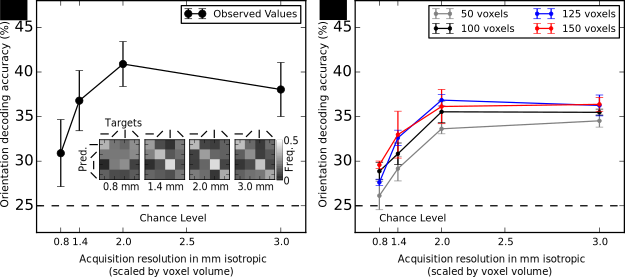
\includegraphics[width=\linewidth]{figure_2}
  \caption{%
    %
    \textbf{(A)} Orientation decoding accuracy on spatially unfiltered data as
    a function of acquisition resolution in the whole contra-lateral V1 ROI.
    Error bars show the standard error of the mean (SEM) across 7 participants
    averaged across hemispheres. Chance level accuracy (25\%) is indicated
    as a horizontal dashed line. Classification performance is detailed in
    confusion matrices for each resolution depicting the frequency of correct 
    classification for each combination of prediction and target values.
    \textbf{(B)} Analog to (A), but with a constant number of input voxels across
    resolutions. 50, 100, 125, or 150 voxels were selected at random from the
    the whole contra-lateral V1 ROI for the classification analysis. Selection was repeated
    100 times. Error bars show SEM across repetitions. Upper range limit of 150
    voxels was determined by the ROI with the least number of voxels at \mm{3} resolution.
    }

    \label{fig:accbyvxsizeandnumber}
\end{figure}


\paragraph*{Time-series signal-to-noise ratio (tSNR)}

It has been shown that overall contrast-to-noise ratio (OCNR) is a factor that
impacts classification performance \citep{chaimow_2011}. According to 
\citet{chaimow_2011} OCNR is a measure is proportional to contrast range and
the square root of the number of voxels and is inversely proportional to 
the noise level. The noise level was calculated as the inverse of 
time course signal to noise ratio (tSNR), which in turn depends on voxel size \citep{triantafyllou_2005}. 
In this study, tSNR is modulated across acquisition resolutions due to differential
impact of technical/thermal and physiological noise components. In order to
characterize this impact, we computed tSNR for each voxel as the ratio of mean
signal intensity across all time points after polynomial detrending
(1\textsuperscript{st} and 2\textsuperscript{nd} order; analog to preprocessing
for MVP analysis) of scanner drift noise and the corresponding standard
deviation. Voxel-wise tSNR was averaged across all experiment runs. For a tSNR
estimate of the whole ROI, we averaged this score across all voxels. The
relationship of voxel volume and tSNR in the empirical data can be well
explained by the following model \citep{triantafyllou_2005}:

$$\text{tSNR}=\kappa  V / \sqrt{1+\lambda^2  \kappa^2  V^2}$$

\noindent where $V$ is the voxel volume, $\kappa$ is the proportionality constant, and
$\lambda$ is the magnetic field strength independent constant parameter with
$\lambda$=0.0117, $\kappa$=22.74 ($R^2$=0.95)  The estimated asymptotic tSNR
limit of $\approx$85 ($\frac{1}{\lambda}$) is similar to the report of
\citet{triantafyllou_2005} for \sevenT\ acquisitions and is reached around
\mm{2.5} acquisition resolution (see Figure~\ref{fig:tSNR_vs_resolution}).

Figure \ref{fig:tsnrsigchange}A illustrates the non-linear relation of tSNR and
orientation decoding accuracy. We observe a substantial drop in accuracy when
decreasing resolution from \unit[2]{mm} to \unit[3]{mm}, despite a further
increase in tSNR.

\begin{figure}
  \centering
  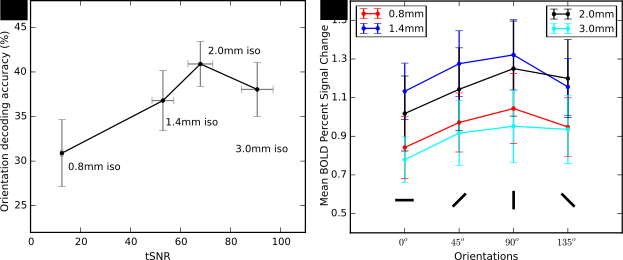
\includegraphics[width=\linewidth]{figure_3}
  \caption{%
    %
    \textbf{(A)} Temporal signal-to-noise ratio (tSNR) as a function of
    resolution (voxel volume). Error bars show the SEM for tSNR and
    accuracy across subjects and hemispheres.
    %
    \textbf{(B)} Estimated BOLD signal change by orientation for all
    resolutions. Maximum pairwise signal change difference is observed
    for the cardinal directions 0\textdegree and 90\textdegree. This
    pattern is congruent with the confusion plots in
    Figure~\ref{fig:accbyvxsizeandnumber}A.}

    \label{fig:tsnrsigchange}
\end{figure}


\paragraph*{BOLD signal change}

Another potential source of differences in orientation decoding accuracy across
resolutions are BOLD signal amplitude differences due to, for example,
differential impact of a partial voluming effect \citep[see][]{tong_2012,
alink_2013}. In order to quantify this effect, we calculated mean percentage
BOLD signal change in response to any flickering orientation stimulus across
resolutions using FeatQuery in FSL \citep[v5.0.8; ][]{Smith_2004}. Similar to 
preprocessing in MVP analysis, no spatial smoothing was performed before 
calculating the percentage signal change. We found
that the mean percentage BOLD signal change was the highest for \mm{1.4} resolution 
(\mm{0.8}: 1.10\%, \mm{1.4}:1.42\%, \mm{2.0}: 1.34\%, and \mm{3.0}: 1.06\%).

In addition, it may also be that particular orientation stimuli elicit stronger
BOLD responses than others \citep[e.g., a grating along the cardinal
orientations;][]{furmanski_2000}.
In order to test for a differential effect and a possible interaction between
orientation and acquisition resolution, we computed a 2-factor (orientation and
resolution) within-subject ANOVA for the estimated BOLD signal change from
all 7 subjects (Figure \ref{fig:tsnrsigchange}B). 
%Mauchly's test indicated that the sphericity assumption was violated for the main effect of orientations
%($W$=0.043, $\chi^2$(5)=14.88, p=0.01); therefore, we report Greenhouse-Geisser corrected test statistics ($\epsilon = 0.405$). 
There was a significant main effect of acquisition resolution ($F$(3, 18)=4.774, p=0.01)
and orientation, $F$(1, 6)=7.581, p=0.03), but no interaction between
the factors, resolution, and orientation ($F$(3, 18)=2.491, p=0.093).


\paragraph*{Impact of head motion on decoding accuracy}
%
Head motion is a likely factor to impact decoding accuracy. In order to
evaluate this effect, we calculated a head motion index suggested by
\citet{alink_2013} for every participant and acquisition resolution. 
%~ In order to yield results comparable to \citet{alink_2013}, we followed their procedure
%~ and excluded subject with very high head motion indices from the analysis (s3
%~ for \mm{0.8}, s6 for \mm{1.4}, s2 for \mm{2.0}, and s3 and s6 for \mm{3.0}).
%
We found a consistent, but non-significant trend towards a negative correlation 
between head motion and decoding accuracy across acquisition resolutions.
(\mm{0.8}: r=-0.45, p=0.3; \mm{1.4}:r=-0.64, p=0.11; \mm{2.0}: r=-0.68, p=0.09; \mm{3.0}: r=-0.23, p=0.6).
%
%~ Without the exclusion of subjects with substantial head movement, the
%~ correlation magnitude was reduced and was not significantly
%~ different from zero for any resolution.


\subsection*{Filtering Strategies}

\paragraph*{Impact of Gaussian smoothing}
%
Figure \ref{fig:spatial_smoothing} A-D show the impact of Gaussian filtering on
the classification performance for data from all four acquisition resolutions.
LP spatial filtering is most commonly performed as a noise reduction step in
fMRI data pre-processing. The classification performance achieved on HP
filtered data of the same filter size is an indication of the amount of usable
information removed by LP filtering. Classification performance on BP filtered
data indicates whether usable information is present in a particular band of
spatial frequencies. Likewise, band-stop performance indicates the presence of
usable information anywhere, except in a particular band.

Except for \mm{0.8} and \mm{1.4} data, LP filtering did not aid classification
performance, relative to the performance on unfiltered data. For all
resolutions, except for \mm{0.8}, the best performance was achieved by LP
filtering with kernel sizes no larger than \mm{3} FWHM.
%
Peak performance on HP filtered data was achieved for filter sizes larger than
\mm{9} FWHM, except for the \mm{0.8} acquisition resolution.
%
BP filtering yielded peak performance for all acquisition resolutions in the
\mm{1}-wide bands in the range of \bandofinterest.
%
Classification performance of BS filtered data remained above-chance for all
spatial frequency bands. The BS performance curve initially follows the LP
performance for small filter sizes, but resembles the HP performance for larger
filter sizes.


\begin{figure}
  \centering
  \includegraphics[width=\linewidth]{figure_4}

  \caption{
    %
    Orientation decoding accuracies for all acquisition resolutions (increasing
    acquisition voxel size from top to bottom) and levels of spatial high-pass,
    low-pass, band-pass, and band-stop Gaussian filtering. Panels on the right
    visualize the size of selected Gaussian filter kernels with respect to the
    voxel size at each resolution. FWHM values for band-pass and band-stop
    filters refer to the corresponding \mm{1} band to the closest smaller
    filter size (e.g., \mm{5} refers to the \mm{4-5} band).
  }
  \label{fig:spatial_smoothing}
\end{figure}



\paragraph*{Impact of spatial resampling to other resolutions, with and without
Gaussian smoothing}
%
As an alternative approach to Gaussian LP filtering for simulating a resolution
reduction, data acquired in a particular resolution were resampled (FFT-based
transformation) to all other resolutions and classification analysis was
performed with and without additional prior Gaussian LP filtering, as suggested
by \cite{freeman_2013}.

Decoding performance on downsampled data was lower than the accuracy obtained from data
recorded in the respective native resolution. Gaussian LP filtering prior to
downsampling generally did not make the decoding accuracies better than 
that of the native resolution data.

Data acquired at \mm{2.0} and \mm{3.0} resolutions, showed a general 
trend of better performance after resampling (upsampling or downsampling)
even with prior Gaussian LP filtering of different kernel sizes. \mm{0.8} 
data consistently showed low decoding accuracy while resampled to any other 
resolution with or without Gaussian filtering. 

%~ any resolution change (upsampling or downsampling) had little effect on the
%~ performance rank across all target resolutions --- with the exception of
%~ upsampling to the highest resolution of \mm{0.8}. Likewise, for any tested
%~ Gaussian LP filter size, decoding on \mm{2} data yielded peak performance with
%~ respect to all other acquisition resolutions.


\begin{figure}
  \centering

    \includegraphics[width=\linewidth]{figure_5}
  \caption{Orientation decoding performance on fMRI data resampled to other
    spatial resolutions, with and without different levels of prior low-pass
    Gaussian spatial filtering. Recording high-resolution data with subsequent
    spatial down-sampling showed a consistent trend of lower classification accuracy
    compared to the native resolution acquisition, with or without prior
    Gaussian low-pass filtering of any tested kernel size.}
    \label{fig:resample}
\end{figure}


\subsection*{Aliasing}

\noindent In the case of frequency aliasing, a (spatial) source frequency is aliased into
a lower frequency when the sampling frequency is too low (Nyquist-Shannon
sampling theorem). If aliasing occurs, the apparent frequency is dependent on
the sampling frequency. We investigated which frequency bands (each \mm{1}
wide) were most informative for orientation decoding across all acquisition
resolutions using Gaussian BP filtered data (Figure \ref{fig:spatial_smoothing}
A-D; orange curves). Peak accuracy was consistently located in the
\bandofinterest\ bands (highlighted range).


\subsection*{Vascular contribution to orientation decoding}
%

\noindent Orientation decoding was performed inside and outside the vein
localizer mask in order to evaluate the availability of orientation
discriminating signal in the vascular system. Two different, arbitrary
thresholds were used to classify voxels as intersecting vs.~nonintersecting
with veins, based on the co-registered and re-sliced vein mask: the top 40\%
and top 10\% of voxels with the highest value after realignment and
reslicing to the target resolution with trilinear interpolation. The resulting
number of voxels is presented in Table~\ref{tab:roisize}.

Decoding accuracy was computed inside and outside the vein mask within the V1
ROI. Analyses outside the vein mask were performed twice: once for the entire
region and again for a subset of voxels that was constrained to the number
of voxels inside the vein mask for the corresponding resolution. In the latter
case, the analysis was repeated with a new random voxel selection 100 times.

Figure~\ref{fig:venous_voxels} shows that with increasing volumetric
homogeneity (smaller voxels, higher threshold) the decoding accuracy approaches
chance-level for ``vein voxels'' while it remains above chance for voxels
outside the vein mask with equivalent thresholds and number of input voxels.



\begin{figure}
  \centering
  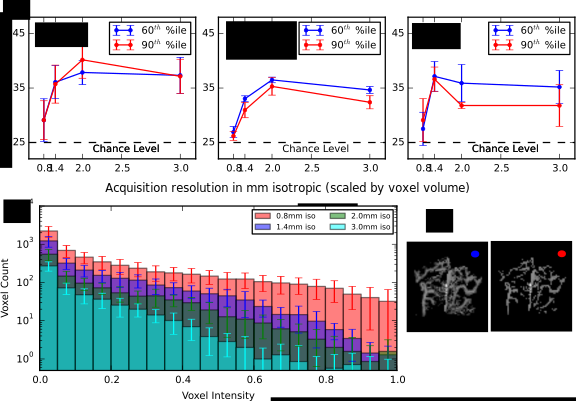
\includegraphics[width=\linewidth]{figure_6}
  \caption{%
    %
    \textbf{(A)} Decoding accuracy was computed inside and outside the vein mask within the V1
    ROI. The vein masks obtained from susceptibility weighted imaging were thresholded
    at two different levels i.e. 60 percentile(\%ile) and 90 percentile(\%ile).
    The panel on the left shows the performance of the entire V1 ROI outside the vein mask (non-venous voxels) 
    for the two different thresholds. Orientation decoding accuracy on V1 voxels restricted to the 
    veins mask (venous voxels) is shown on the right panel. The middle panel 
    depicts the decoding performance of a fixed number of non-venous voxels, 
    the number of voxels being equal to the number of venous voxels in the right panel 
    corresponding to every resolutions and thresholds. The dashed horizontal lines indicate the chance performance.
    \textbf{(B)} Trilinear interpolation was used to reslice the vein mask to all
    four target resolutions. The histogram shows the distribution of mask voxel
    intensities corresponding to the volumetric fraction of ``vein voxels'' in
    the high-resolution vein mask (voxel count axis in log-scale).
    \textbf{(C)} Axial maximum intensity projection of the vein mask of one participant
    resliced to the \mm{0.8} resolution; illustrates the two chosen thresholds. The color indicator correspond to the curves depicted in panel A.
    }
    \label{fig:venous_voxels}
\end{figure}


\section*{Discussion}

\noindent In order to determine optimal spatial acquisition and spatial filtering
parameters for the decoding of visual orientations from fMRI data recorded from
visual cortex, we measured ultra-high field \sevenT\ fMRI data in four
different resolutions from 7 participants. Linear SVM classifiers were trained
to classify voxel patterns of regression weights of hemodynamic response models
for the visual stimulation with four different oriented gratings.
Cross-validated classification accuracy was used as quality metric.

The overall classification accuracies reported here are relatively low (peaking
at $\approx$50\% with a theoretical chance-level performance of 25\% for the
4-way classification analyses employed in this study). This indicates that
either the orientation-specific signal in the BOLD fMRI data is relatively
noisy and the acquired amount of data is insufficient for appropriate
classifier training, or that a linear decision boundary (in contrast to a
non-linear decision surface) is a suboptimal classification model, or both.
Similar studies in the literature have often used binary classification
paradigms \citep[for example,][]{alink_2013, chaimow_2011} or reported average
pairwise accuracy for classification performance results like \citep[e.g.,
][]{kamitani_2005,opdebeeck_2010}. Converted into average pairwise binary
accuracies, the results reported here range from 55\% to 70\% (for \mm{0.8} and
\mm{2} respectively, each accuracy corresponding to an analysis of the full V1
ROI and with no additional smoothing; see
Figure~\ref{fig:accbyvxsizeandnumber}A; theoretical chance-performance: 50\%),
hence accuracies are of the same magnitude as in other studies \citep[see, for
example, ][]{haynes_2005,alink_2013}. Therefore, we conclude that the overall
quality of the present data is comparable to that of previous studies, and that
the results presented here can be used to address open questions regarding the
impact of data acquisition and spatial filtering parameters on the decoding of
orientation from the early visual cortex.

\paragraph*{Optimal acquisition resolution}
%
Among the four tested acquisition resolutions, the highest decoding accuracy is
achieved with a \mm{2} resolution (Figure~\ref{fig:accbyvxsizeandnumber}A).
Under the assumption of a quadratic relation of accuracy and resolution, an
optimal resolution is estimated to be at $\approx$\mm{2.5} isotropic
voxel size. This result is congruent with a simulation study by
\citet{chaimow_2011} that analyzed the impact of anatomical and physiological
properties of primary visual cortex, as well as technical parameters of BOLD
fMRI acquisition on the accuracy of decoding the stimulated hemifield from
signal sampled from ocular dominance columns. The study includes a number of
predictions for choosing optimal voxel size and number of input voxels to
maximize decoding accuracy for \threeT\ fMRI \citep[see Figure 6
in][]{chaimow_2011} that show a striking similarity to the results presented
here (Figure~\ref{fig:accbyvxsizeandnumber}). For \threeT\ fMRI,
\citet{chaimow_2011} showed that peak decoding accuracy is achieved at around
\mm{3} isotropic voxel size. In line with our hypothesis, we find that the
optimal resolution for the decoding of visual orientations from \sevenT\ fMRI
data is higher than that. Likely reasons are a higher spatial frequency
profile of orientation columns compared to ocular dominance columns
\citep[see][for evidence from monkeys]{obermayer_1993} and the considerably
smaller BOLD PSF at \sevenT\ compared to \threeT\ \citep[\mm{$\approx$2.3} FWHM
vs. \mm{$\approx$3.5} FWHM][]{shmuel_2007, engel_1997}.

Superior decoding performance at \mm{2} could still be observed even when the
number of input voxels for classification is held constant across resolutions,
although the performance differences between resolutions are reduced
(Figure~\ref{fig:accbyvxsizeandnumber}B). The ratio of input features (voxels)
and the number of observations (fixed in this study) is a critical factor for
the training of a classification model, as with increasing dimensionality the
sampling of the feature space becomes sparser, and, consequently, the estimated
decision surface suffers from increased uncertainty \cite[curse of
dimensionality, ][after \citealt{friedman2001elements}]{bellman1961adaptive} In
this study, the number of voxels in the ROI varies by a factor of $>$20 from
the lowest to the highest resolution (Table~\ref{tab:roisize}). The pattern of
decoding accuracy differences when using the full ROI vs.~a constant number of
voxels across all resolutions could indicate that $\approx$700 input voxels
(size of the ROI at \mm{2}) represents the optimal trade-off between the number
of observations and input voxels, given the noise in the data and the fixed
number of observations in this study.

Moreover, the present data suggest, in line with \citet{chaimow_2011}, that
temporal signal-to-noise-ratio, an indicator of temporal signal stability, is a
critical factor for optimal decoding accuracy
(Figure~\ref{fig:tsnrsigchange}A). In contrast, the overall BOLD signal change
amplitude does not seem to be predictive for decoding accuracy (for example,
\mm{0.8} and \mm{2} data show very similar orientation-specific signal change
patterns despite markedly different decoding performance;
Figure~\ref{fig:tsnrsigchange}B).


\paragraph*{Optimal low-pass filter size}
%
Gaussian spatial LP filtering is one of the most common preprocessing steps for
fMRI data analyses. However, the present findings indicate that explicit
spatial LP filtering, in addition to the implicit spatial filtering due to
inherent motion, and the effect of head movement correction algorithms is
generally not beneficial for orientation decoding
(Figure~\ref{fig:spatial_smoothing}). Only for resolutions higher than \mm{2}
does additional spatial smoothing with \mm{2-3} FWHM show a tendency for improved
decoding accuracy. This suggests that, given a resolution, a spatial
smoothness equivalent to a Gaussian kernel size of \mm{$\approx$2} FWHM is
optimal. This is congruent with the observation of overall lower decoding
accuracies for \mm{3} scans and is in line with the prediction of the quadratic
model of acquisition resolution and decoding accuracy presented above.

Moreover, LP filtering by means of spatial down-sampling is not beneficial for
orientation decoding either. As shown in Figure~\ref{fig:resample} (\mm{0} data
points, corresponding to no Gaussian smoothing), orientation decoding on
down-sampled data never outperforms the decoding on data natively recorded in
the corresponding resolution.


\paragraph*{Spatial characteristics of orientation specific signals}
%
The analysis of individual spatial frequency bands (BP filter, \mm{1} width;
Figure~\ref{fig:spatial_smoothing}) revealed that orientation-related signal is
present in a wide range of bands as indicated by above-chance decoding
performance for nearly all tested bands. However, a drop in decoding accuracy
can be observed across all resolutions for bands from \mm{$\approx$12} and all
lower frequencies. This indicates that large scale orientation-related signal
biases, as suggested by some authors \citep{opdebeeck_2010,freeman_2011}, exist,
but do not represent the most pronounced information usable for orientation
decoding. This interpretation is consistent with the finding that orientation
decoding on spatially down-sampled data with prior removal of high-frequency
components, as suggested by \cite{freeman_2013} as a test for the contribution
of fine-scale signals, reveals decreasing decoding performance with increasing
LP filter size (Figure~\ref{fig:resample}).
%
The observation that for filter sizes \mm{8-10} and larger, performance on HP
filtered data plateaued and the BP filtered data showed better performance than
the LP filtered components in all resolutions, signals that low spatial
frequency fMRI components have a negative impact on decoding accuracy.

\cite{carlson_2014} identified neuronal activity patterns related to stimulus
edges that mimic a radial bias as a potential source of a global signal bias.
The stimuli employed in this study had clearly visible, unsmoothed edges, hence
edge-related activity is a valid explanation for the observed
orientation-related large-scale signals.

Overall, BP filtering yielded peak performances for all resolutions, indicating
that both high and low spatial frequency components contribute less to
orientation decoding. Consistent with \citet{alink_2013}, the present results
suggest that the \mm{$\approx$5-8} band carries the most orientation-related
signal. The Nyquist-Shannon Sampling Theorem dictates that, in order to measure
a particular signal appropriately, the sampling frequency has to be at least
twice the critical frequency of that signal. Given a \mm{$\approx$5-8} band, a
minimum sampling frequency wavelength of \mm{$\approx$2.5} is required to
measure the corresponding spatial frequencies without aliasing. This estimate
is consistent with the predictions of the quadratic model of the relation of
acquisition resolution and decoding performance. The observed lower accuracy
for \mm{3} data vs.~\mm{2} data could, thus, be explained by an insufficient
sampling frequency, whereas the nearly identical peak performance of \mm{1.4}
and \mm{2} is compatible with this minimum frequency rule. However, the
markedly lower decoding performance on \mm{0.8} data is evidence that a minimum
sampling resolution of \mm{$\approx$2.5} is necessary but not sufficient for
optimal decoding performance. It indicates that an optimal balance of scanning
resolution and temporal signal-to-noise-ratio is reached at \mm{$\approx$2.5},
scanning at higher resolution reduces tSNR and scanning at lower resolutions
does not allow sampling the underlying higher frequency neuronal activation
patterns.


\citet{alink_2013}, \citet{gardner_2010} and \citet{kriegeskorte_2010} argued
that the high spatial frequency signal of orientation columns in early visual
cortex could be reflected in (much larger) fMRI voxels by means of spatial
aliasing (hyperacuity). The present data does not support this hypothesis. In
the case of frequency aliasing due to an insufficient sampling frequency, the
frequency of the aliased signal would vary depending on the actual sampling
frequency.  However, the peak decoding performance is always located in the
\bandofinterest\ band across all four resolutions. This finding alone does not
rule out the representation of an aliased columnar signal,
but it suggests that, even if such a signal exists, it does not determine peak
orientation decoding performance.

This interpretation is in line with \citet{kamitani_2005} and
\citet{chaimow_2011} which show that the spatial frequencies of columnar structures (0.5
cycles/mm) do not contribute signal for decoding, due to several technical
limitations like inherent head motion and reduced SNR proportional to reduction
in voxel volume.  Moreover, \citet{shmuel_2007} state that the PSF --- that
captures blurring factors due to eye movements, neuronal response, BOLD
response PSF in gray matter, as well as the PSF of the data acquisition process
--- makes fMRI data inherently LP filtered and, as such, poses a physical
limitation on the spatial frequency scale from which fMRI signal can be
obtained. \citet{kamitani_2005} and \citet{chaimow_2011} identify contributions
from random variations and irregularities in the columnar structures captured
by larger voxels as the main source of information for decoding.  These are of
considerably lower frequency than the primary spatial frequency
characteristics of the columnar organization and are lower than the Nyquist
criterion of the BOLD fMRI sampling frequencies.

It could be speculated that the spatial scale of the orientation signal as
estimated by volumetric spatial filtering is, to some degree, determined by the
representation of the cortical folding pattern in the scan volume.
Figure~\ref{fig:distance_plot} illustrates that a BP filter corresponding to
the most informative spatial frequency band is of sufficient size to average
signal across the entire diameter of the folded calcarine sulcus, whereas a
smaller filter is not, and a bigger filter includes a substantial fraction of
the surrounding white matter and adjacent cortical fields. Further
studies should relate the optimal volumetric filter size to the regional
variability of the cortical folding pattern \cite[see, for
example,][]{germanaud_2012} or compare the current findings with analyses
performed on data projected onto the cortical surface.

\begin{figure} \centering
  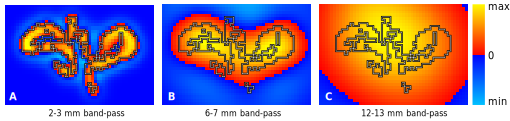
\includegraphics[width=\linewidth]{figure_7}
  \caption{
    %
    Illustration of the band-pass filtered ROI mask (coronal slice) of the
    first participant for three spatial frequency bands corresponding to higher
    (A), matching (B), and lower (C) frequencies relative to the most
    informative band for orientation decoding. The outline shows the boundaries
    of the original V1 mask. The relative scaling of the maps can be
    interpreted as the fraction of signal in the spatial band that originates
    from inside the volumetric ROI. For the most informative band, the filter
    size approximately matches the volumetric width of the ROI across cortical
    boundaries.
   %
  }

    \label{fig:distance_plot}
\end{figure}


\paragraph*{Venous voxels in V1 ROI contribute above chance classification of
orientation gratings}
%
Several authors have cited the potential presence of an orientation-related
BOLD response pattern originating from the vascular system (draining veins) as
a potential signal that is picked up by a classification model and that is
potentially able to introduce spatial biases in the representation of
orientation \citep{kriegeskorte_2010, chaimow_2011, shmuel_2010}. The present
results seem to suggest that a signal originating from draining veins is very
weak, if it exists at all. With increasing homogeneity and more rigorous
thresholds for classifying voxels as ``intersecting with veins'', the decoding
performance drops to chance-level while it remains above chance in comparison
analyses with an equal number of non-venous voxels. Given this finding, it is
unlikely that draining veins contribute to a spatial distortion of
orientation-related BOLD signal with respect to the underlying distribution of
neural activity.


\paragraph*{Limitations}

The focus of the present study was to investigate the effect of acquisition
resolution and spatial filtering on the decoding of visual orientations from
primary visual cortex. In order to yield comparable results, the acquisition
parameters were constrained to guarantee a certain minimum coverage of the V1
ROI even at the highest resolutions and to have an identical temporal sampling
frequency (TR) to yield the same number of observations across all resolutions.
This choice implied that the GRAPPA acceleration factor had to be increased
with increasing resolution, hence leading to an increased under-sampling of the
k-space with higher resolutions. This could impact the sensitivity of the scan
to high-frequency spatial signals. A future study will have to test whether the
present findings hold when constraints on coverage and sampling frequency are
relaxed. For example, a study by \cite{demartino2013grase} using a 3D gradient
and spin echo (GRASE) sequence suggests that such a sequence outperforms a
gradient echo sequence, such as the one employed in this study, for
high-resolution imaging at \mm{0.8} isotropic resolution --- at the expense of a
vastly reduced scan volume.

The present study is exclusively based on \sevenT\ fMRI data, hence it remains
unclear in which way the characteristics of the relation of decoding
performance and acquisition resolution are dependent on MR field-strength. The
differences in the sizes of the BOLD point-spread functions
\citep{shmuel_2007,engel_1997} suggest a lower resolution limit for \threeT\
scans. However, the reported optimal resolution is within the range of
conventional acquisition resolutions of today's \threeT\ scanners. A future
study should address the question of how the decoding performance varies with
field-strength for identical resolutions.

While this study focused on the optimal acquisition parameters for decoding of
visual orientation from fMRI BOLD response patterns in early visual cortex, we
found empirical evidence that these parameters are primarily determined by
technical and physiological properties of the acquisition method rather than
fine-scale spatial characteristics, \eg columnar, of the underlying neural signal.
Consequently, it can be hypothesized that optimal settings for other decoding
paradigms and cortical areas may be similar in nature. Further simulation
studies for sensory systems and multi-resolution acquisitions for other
stimulation paradigms are required to test the generality of these findings.

\subsection*{Conflict of interest}

\noindent The authors declare no competing interest.
